\documentclass[12pt,a4paper,ngerman]{article}
\usepackage[top=2.5cm, bottom=2cm, left=2.5cm, right=2.5cm]{geometry} 
\usepackage[utf8x]{inputenc}
\usepackage{ngerman}
\usepackage{lmodern}
\usepackage{listings}
\usepackage{amssymb,amsmath}
\usepackage{ifxetex,ifluatex}
\usepackage{fixltx2e} % provides \textsubscript
% use microtype if available

% Redefine labelwidth for lists; otherwise, the enumerate package will cause
% markers to extend beyond the left margin.
\makeatletter\AtBeginDocument{%
  \renewcommand{\@listi}
    {\setlength{\labelwidth}{4em}}
}\makeatother
\usepackage{enumerate}
\usepackage{graphicx}
% We will generate all images so they have a width \maxwidth. This means
% that they will get their normal width if they fit onto the page, but
% are scaled down if they would overflow the margins.
\makeatletter
\def\maxwidth{\ifdim\Gin@nat@width>\linewidth\linewidth
\else\Gin@nat@width\fi}
\makeatother
\let\Oldincludegraphics\includegraphics
\renewcommand{\includegraphics}[1]{\Oldincludegraphics[width=\maxwidth]{#1}}
\ifxetex
  \usepackage[setpagesize=false, % page size defined by xetex
              unicode=false, % unicode breaks when used with xetex
              xetex]{hyperref}
\else
  \usepackage[unicode=true]{hyperref}
\fi
\hypersetup{breaklinks=true,
            bookmarks=true,
            pdfauthor={},
            pdftitle={},
            colorlinks=true,
            urlcolor=blue,
            linkcolor=magenta,
            pdfborder={0 0 0}}
\setlength{\parindent}{0pt}
\setlength{\parskip}{6pt plus 2pt minus 1pt}
\setlength{\emergencystretch}{3em}  % prevent overfull lines
\setcounter{secnumdepth}{0}

\title{Enterprise Integration Patterns in dem Praxis mit Apache Camel
und Spring Integration}
\author{Anders Malmborg und Michael Haslgrübler}
\date{}

\lstset{ %
numbers=left,                   % where to put the line-numbers
basicstyle=\itshape,
numberstyle=\scriptsize,      % the size of the fonts that are used for the line-numbers
stepnumber=1,                   % the step between two line-numbers. If it's 1 each line will be numbered
numbersep=5pt,                  % how far the line-numbers are from the code
backgroundcolor=\color{white},  % choose the background color. You must add \usepackage{color}
showspaces=false,               % show spaces adding particular underscores
showstringspaces=false,         % underline spaces within strings
showtabs=false,                 % show tabs within strings adding particular underscores
%extendedchars=false,
frame=single,			% adds a frame around the code
tabsize=2,			% sets default tabsize to 2 spaces
captionpos=b,			% sets the caption-position to bottom
breaklines=true,		% sets automatic line breaking
breakatwhitespace=false,	% sets if automatic breaks should only happen at whitespace
escapeinside={\%*}{*)}          % if you want to add a comment within your code
}

\begin{document}

\maketitle

\section{Einleitung}

Derzeit zeichnet sich ein Trend weg von monolithischen in Richtung
modularen Systemen ab, wurde bisher der gesamte Anwendungslogik von
einem System zur Verfügung gestellt, werden zunehmend fachliche
Teilprozesse in sowohl Architektur, Entwicklung und Betrieb geteilt
betrachtet. Für den Endanwender erscheint es als ein Produkt, die
``Nahtstellen'' sind nicht sichtbar. Mit {[}Microservices{]}
{[}microsvc{]} haben einige Unternehmen wie Amazon oder Netflix für
Aufmerksamkeit gesorgt. Diese modularen Systeme versprechen Vorteile vor
allem in der Skalierbarkeit und Unabhängigkeit bei der Entwicklung der
Teilprodukte.

Obwohl Microservices es nicht zwangsweise benötigten, setzt sich auch
ein weiteres Architekturmuster für die Skalierbarkeit durch, nämlich die
{[}ereignisbasierte Architektur{]} {[}ea{]} wo Verarbeitungsschritte
asynchron und parallel erfolgen.

Mit oder ohne modularer und/oder ereignisbasierter Architektur kommt man
heutzutage an der Integration mit externen Systemen nicht vorbei, es
werden synchrone Schnittstellen über WebServices als auch der asynchrone
Datenaustausch in diversen Produkten nicht mehr wegzudenken, z.B.: Login
via Facebook, Rechnungsmeldung zum Finanzamt, \ldots{}

\begin{figure}[htbp]
\centering
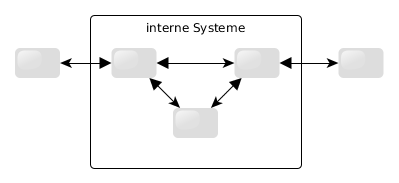
\includegraphics{systems.png}
\caption{Interne und externe Systeme}
\end{figure}

Für die Interaktion zwischen internen als auch externen Systemem findet
man im Buch {[}Enterprise Integration Patterns{]} {[}eip{]}
Lösungsmustern, welche für eine Vielzahl von Problemen die durch diese
Interaktion entstehen angewandt werden. Diese Enterprise Integration
Patterns wurden in den Frameworks {[}Apache Camel{]} {[}camel{]} und
{[}Spring Integration{]} {[}si{]} umgesetzt und werden in diesem Artikel
anhand eines Praxisbeispiels erklärt und durchleuchtet.

Anhand des Fahrradshop, wird gezeigt wie man beide Frameworks einsetzen
kann und typische Integrationsszenarien lösen kann.

\section{Enterprise Integration Patterns}

Die wichtigsten und häufigsten Integrationsmustern sind folgende 4 Arten
(Styles): File Transfer, Shared Database, Remote Procedure
Invocation/Call (RPC) und Messaging.

Im fiktiven Fahrradshop werden drei der vier Integrationsmuster (File
Transfer, Remote Procedure Invocation und Messaging) anhand vom
praxisorientierten Problemen eingesetzt.

\subsection{File Transfer und Shared Database}

File Transfers sind relativ einfach zu implementieren, bietet aber keine
Möglichkeit synchrone Kommunikation damit zu implementieren.

Shared Database kann für einfache Fälle überlegt werden. Mit wachsenden
Anzahl der beteiligten Systeme wird die enge Kopplung über Datenbank
aber zu Problemen führen und es eignet sich außerdem oft nicht für die
Kommunikation über Unternehmensgrenzen hinweg.

\subsection{Remote Procedure Invocation und Messaging}

Mit Remote Procedure Invocation und Messaging stehen anderseits
skalierbare Lösungen für synchrone bzw. asynchrone Kommunikation zur
Verfügung. Durch sogenannte Message Channels wird die Kommunikationsart
abstrahiert und von der fachlichen Implementierung abgekoppelt. Das
heißt das sofern sich die Anforderung ändern auch die Möglichkeit
besteht auf Konfigurationsbasis den Kommunikationsmechansismus zu ändern
ohne sein Produkt neu entwickeln zu müssen.

Messaging wird verwendet um zuverlässig und zeitnah Daten zwischen den
Services auszutauschen. Bei asynchronen Schnittstellen werden die Daten
über einen kürzeren oder längeren Zeitraum zwischengespeichert. Damit
wird das Gesamtsystem fehlertoleranter - da nicht alle Services
gleichzeitig zur Verfügung stehen müssen.

\begin{figure}[htbp]
\centering
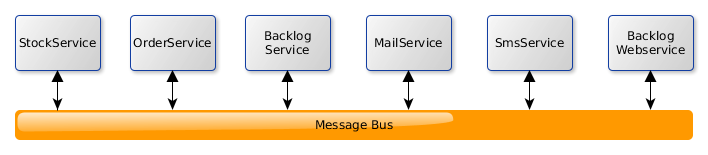
\includegraphics{messaging.png}
\caption{Messaging}
\end{figure}

Messages werden über Channels geschickt. Der Absender und Empfänger
verbinden sich mit dem Channel. Falls es ein Absender und genau einen
Empfänger gibt wird ein Point-to-Point Channel verwendet, ansonsten, bei
mehreren Empfänger, für einen Message bietet sich der Publish-Subscribe
Channel an.

Der Empfänger kann auch zur Laufzeit entschieden werden. In unserem
Beispiel sollte nach der Verarbeitung des Auftrages eine Nachricht an
den Kunden verschickt werden. Je nach Kunde sollte entweder eine SMS
oder eine Mail verschickt werden. Die Entscheidung ob das Message zum
SmsService oder MailService weitergereicht werden sollte, trifft hier
ein Content-Based Router.


\begin{figure}[htbp]
\begin{center}
\Oldincludegraphics[height=10cm]{channels.png}
\end{center}
\caption{Channels}
\end{figure}

Nach diesem sehr gekürzten Übersicht von Enterprise Integration Patterns
stellen wir jetzt die Anwendung vor.

\section{Architekturmodell des Shops}

\begin{figure}[htbp]
\centering
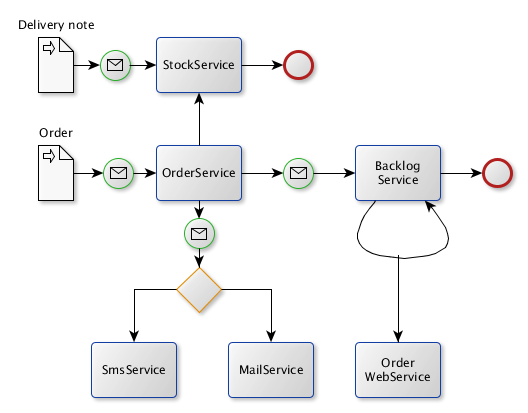
\includegraphics{eip.png}
\caption{EIP im Fahrradshop}
\end{figure}

Bei einer Bestellung wird zuerst geprüft ob eine ausreichende Menge des
gewünschten Artikels im Lager des Fahrradshops vorhanden ist. Im Lager
vorhandene Artikel werden ausgebucht und die fehlende Menge wird
nachbestellt. Die Lieferanten senden Lieferscheine, die als
Lagereingänge behandelt werden.

Das Architekturmodell in Kürze:

\begin{itemize}
\item
  StockService: verwaltet Lagerbestände. Lieferscheine von externen
  Lieferanten werden als CVS-Dateien eingespielt.
\item
  OrderService: verwaltet Bestellungen. Stellt REST basierte
  Schnittstellen für eine Browserapplikation zur Verfügung.
\item
  BacklogService: bestellt auf Lager fehlende Artikeln bei externen
  Lieferanten die SOAP Webservices dafür zur Verfügung stellen.
\item
  Sms- bzw. MailService: sendet Bestellbestätigungen an den Kunden über
  SMS oder Mail.
\end{itemize}

Die Services werden so entwickelt, dass keine enge Kopplung besteht. Sie
können damit in separaten Laufzeitumgebungen auf unterschiedlichen
Servern betrieben werden.

\subsection{Use Cases}

\paragraph{CSV Import von Lieferscheine}

Die Lieferscheine werden als CSV Dateien aus einem Verzeichnis gelesen.
Eine Zeile beinhaltet Typ, Bezeichnung, Teilenummer, Einkaufspreis sowie
Anzahl gelieferte Teile:

\begin{lstlisting}
FRAME; Road bike frame 60 cm;1935182366;103.95;2
DRIVE; Shimano HG LX;1935182439;31.85;6
\end{lstlisting}

Die Verarbeitungsschritte:

\begin{enumerate}[1.]
\item
  Zeilenweise einlesen
\item
  In Typ, Bezeichnung u.s.w aufteilen
\item
  Lagerbestände korrigieren
\end{enumerate}

\paragraph{Bestellabwicklung}

Der Kunde stellt eine Warenkorb im Browser zusammen. Der Kunde sollte
nach der Bestellannahme eine Bestätigung erhalten. In einer
Systemkonfiguration ist hinterlegt ob der Kunde mittels SMS oder Mail
die Bestätigung erhalten soll. Senden der Bestätigung sollte asynchron
von der Verarbeitung stattfinden da die Bestätigung nicht so hohe
Priorität wie (neue) Bestellungen hat.

\begin{enumerate}[1.]
\item
  Prüfen ob bestellte Artikeln auf Lager sind:

  \begin{itemize}
  \item
    falls nicht einen Bestellwunsch erzeugen
  \item
    Andernfalls den Lagerbestand reduzieren
  \end{itemize}
\item
  Bestätigung senden
\end{enumerate}

\paragraph{Nachschub fehlende Artikeln}

Sofern bestellte Artikeln nicht lagernd sind, werden sie mittels
Webservices von externen Lieferanten nachbestellt.

\section{Umsetzung mit Spring Integration und Channel}

Beide Frameworks unterstützen die Mustern von Enterprise Integration
Patterns und beziehen sich auch auf das Buch in der Dokumentation.
Fallweise werden andere Namen verwendet, Spring Integration verwendet
Beispielsweise Direct Channel statt Point-to-Point Channel.

Für die asynchrone Austausch von Nachrichten verwenden wir {[}Apache
ActiveMQ{]} {[}amq{]}. Beide Frameworks integrieren problemlos mit
ActiveMQ.

\subsection{Anmerkung zu der Konfiguration von Spring Integration und
Apache Camel}

Spring Integration unterstützt ``klassische'' Spring XML Konfiguration
als auch Annotationen. Apache Camel unterstützt Spring Konfiguration mit
oder ohne Annotationen. Weiter kann Camel mit Java DSL statt oder
zusätzlich zur Spring XML Konfiguration verwendet werden. Zwecks
Vergleichbarkeit der beiden Frameworks wird hier immer nur Spring XML
Konfiguration verwendet.

\subsection{Java Service Implementierungen}

Die Implementierungen der Services sind völlig unwissend von Spring
Integration bzw. Apache Camel. Hier ein Teil der Implementierung von
OrderService:

public Backlog handleOrder(Order order) \{

\begin{lstlisting}
    List<BacklogItem> backlogItems = new ArrayList<BacklogItem>();
    Customer customer = customerRepository.findByName(order.getCustomerName());
    if (customer == null)
    {
        customer = new Customer(order.getCustomerName());
    }
    customer.getOrders().add(order);
    for (OrderItem orderItem : order.getOrderItems()) {
        orderItem.setStatus(OrderItemStatus.BACKLOG);
        StockItem stockItem = stockService.getStockItem(orderItem.getItem().getNumber());
        if (stockItem != null)
        {
            if (stockItem.getQuantity() > 0) {
                orderItem.setStatus(OrderItemStatus.CHECKED_OUT);
                stockService.checkoutStockItem(stockItem);
                continue;
            }
        }
        backlogItems.add(new BacklogItem(new Item(orderItem.getItem())));
    }
    customerRepository.save(customer);
    return new Backlog(backlogItems);
}
\end{lstlisting}

In der Implementierung ist zu sehen, dass keine Verbindung mit dem
BacklogService besteht.

\paragraph{CSV Import von Lieferscheine mit Spring Integration}

Da in der Spring Familie ausgereifte Funktionalität für CSV Verarbeitung
in Form vom {[}Spring Batch{]} {[}sb{]} vorhanden ist, gibt es keine
eigene Implementierung für CSV in Spring Integration. Die Konfiguration
für Spring Batch

\begin{lstlisting}
<bean id="deliveryNoteCsvReader" class="org.springframework.batch.item.file.FlatFileItemReader"
    scope="prototype">
    <property name="encoding" value="UTF-8" />
    <property name="lineMapper">
        <bean class="org.springframework.batch.item.file.mapping.DefaultLineMapper">
            <property name="lineTokenizer">
                <bean
                    class="org.springframework.batch.item.file.transform.DelimitedLineTokenizer">
                    <property name="delimiter" value=";" />
                    <property name="names" value="itemType,name,number,price,quantity" />
                </bean>
            </property>
            <property name="fieldSetMapper">
                <bean class="eip.spring.integration.StockItemFieldSetMapper" />
            </property>
        </bean>
    </property>
</bean>
\end{lstlisting}

\begin{itemize}
\item
  DelimitedLineTokenizer: teilt jede Zeile in einzelne Felder.
\item
  DefaultLineMapper: lässt den DelimitedLineTokenizer die Zeile zerlegen
  und StockItemFieldSetMapper daraus einen Objekt erzeugen
\item
  FlatFileItemReader: liest die CSV Datei zeilenweise.
\end{itemize}

Da jetzt Spring Batch so weit konfiguriert ist, folgt nun Spring
Integration. Der \emph{inbound-channel-adapter} überwacht einen
Verzeichnis, falls Dateien gefunden werden, werden sie auf die Reise auf
den Channel \emph{csvDeliveryNotesChannel} geschickt.

\begin{lstlisting}
<int-file:inbound-channel-adapter id="deliveryNotesChannelAdapter"
    directory="file:../eip-common/src/main/resources/deliverynotes" channel="csvDeliveryNotesChannel">
    <int:poller fixed-rate="1000" />
</int-file:inbound-channel-adapter>
\end{lstlisting}

Ein "service-activator* horcht auf den \emph{csvDeliveryNotesChannel}
und leitet die Messages(hier Dateien) an den Spring Bean
\emph{deliveryNoteCsvImport} weiter.

\begin{lstlisting}
<int:service-activator input-channel="csvDeliveryNotesChannel"
    ref="deliveryNoteCsvImport" method="importCsv" />
\end{lstlisting}

Die Spring Konfiguration der verwendete Beans:

\begin{lstlisting}
<bean id="deliveryNoteCsvImport" class="eip.spring.integration.DeliveryNoteCsvImport"
    scope="prototype">
    <constructor-arg name="reader" ref="deliveryNoteCsvReader" />
    <constructor-arg name="writer" ref="stockWriterAdapter" />
</bean>

<bean id="stockWriterAdapter"
    class="org.springframework.batch.item.adapter.ItemWriterAdapter">
    <property name="targetObject" ref="stockService" />
    <property name="targetMethod" value="addStockItem" />
</bean>
\end{lstlisting}

Die Java-Implementierung ist minimal, Spring Integration hier
unterstützt von Spring Batch, muss lediglich konfiguriert werden.

\paragraph{Umsetzung mit Apache Camel}

Camel hat eine hohe Anzahl von Komponenten(Components). Diese werden in
Form von URIs konfiguriert. Wir verwenden hier das File Component um den
Verzeichnis für neue Dateien zu überwachen. Der Splitter teilt die Datei
in einzelne Zeilen auf und zerlegt diese in Felder. Der Processor
\emph{csvToStockItemProcessor} erzeugt aus die Felder einen
StockItem-Objekt. Zum Schluss werden die Objekte vom Spring Bean
\emph{stockService} auf der Datenbank gespeichert.

\begin{lstlisting}
<camel:camelContext id="deliveryNoteImport">
    <camel:route>
        <camel:from uri="file://../eip-common/src/main/resources/deliverynotes?consumer.delay=1000&noop=true" />
        <camel:split streaming="true">
            <camel:tokenize token="\n" xml="false" />
            <camel:unmarshal>
                <camel:csv delimiter=";" />
            </camel:unmarshal>
            <camel:process ref="csvToStockItemProcessor" />
            <camel:bean ref="stockService" method="addStockItem"/>
        </camel:split>
    </camel:route>
</camel:camelContext>
\end{lstlisting}

Die Konfiguration für CSV Import ist bei Apache Camel um einiges
kompakter.

\subsection{Entkopplung der Bestellbestätigung mittels Apache
ActiveMQ}

Der Kunde sollte nach der Bestellannahme eine Bestätigung erhalten. In
einer Systemkonfiguration ist hinterlegt ob der Kunde mittels SMS oder
Mail die Bestätigung erhalten soll. Senden der Bestätigung sollte
asynchron von der Verarbeitung stattfinden da die Bestätigung nicht so
hohe Priorität wie (neue) Bestellungen hat. Daher wird ActiveMQ als JMS
Implementierung eingesetzt und dient als Entkopplung zwischen
OrderService und Sms- bzw. MailService.

Weiter sollte der OrderService nicht mit der Entscheidung ob SMS oder
Mail angebracht ist bzw. die dafür notwendige Parametern für SMS oder
Mail Versand beschäftigt werden.

ActiveMQ wird für beide Implementierung gleich konfiguriert:

\begin{lstlisting}
<amq:broker useJmx="false" persistent="false">
    <amq:transportConnectors>
        <amq:transportConnector uri="vm://localhost" />
    </amq:transportConnectors>
</amq:broker>
\end{lstlisting}

\paragraph{Umsetzung mit Spring Integration}

Zuerst wird die Bestellbestätigung \emph{Notification} in entweder einer
\emph{SmsNotification} oder einer \emph{MailNotification} umgewandelt.
Dafür wird einen \emph{Transformer} implementiert:

\begin{lstlisting}
public Message<?> transform(Message<?> message) {
    Notification notification = (Notification) message.getPayload();
    Notification outNotification;
    if (customerConfig.getContactChannel(notification.getCustomer()).equals(SMS))
        outNotification = new SmsNotification(notification.getCustomer(),
                                              notification.getMessage(), 
                                              customerConfig.getSmsNumber(notification.getCustomer()));
    else
        outNotification = new MailNotification(notification.getCustomer(),
                                               notification.getMessage(), 
                                               customerConfig.getMailAddressNumber(notification.getCustomer()),
                                               customerConfig.getMailSubject(notification.getCustomer()));
    return MessageBuilder.withPayload(outNotification).build();
}
\end{lstlisting}

Die Spring Konfiguration schaut wie folgt aus:

\begin{lstlisting}
<int:transformer id="notificationTransformer" input-channel="transformerChannel"
    method="transform" output-channel="routingChannel">
    <bean class="eip.spring.integration.NotificationTransformer" />
</int:transformer>
\end{lstlisting}

Das Versenden erfolgt durch den Sms- bzw. MailService. Dazu wird ein
\emph{Router} verwendet:

\begin{lstlisting}
<int:payload-type-router input-channel="routingChannel">
    <int:mapping type="eip.common.services.SmsNotification"
        channel="smsOutQueue" />
    <int:mapping type="eip.common.services.MailNotification"
        channel="mailOutQueue" />
</int:payload-type-router>
\end{lstlisting}

Die Art der Messages, \emph{SmsNotification} oder
\emph{MailNotification} entscheidet über den zu verwendenden Channel.

Zum Schluss die Konfiguration für die JMS Anbindung . hier für SMS:

\begin{lstlisting}
<int-jms:outbound-channel-adapter id="smsJms"
    channel="smsOutQueue" destination="smsJmsQueue" />

<bean id="smsJmsQueue" class="org.apache.activemq.command.ActiveMQQueue">
    <constructor-arg value="queue.sms" />
</bean>

<int-jms:message-driven-channel-adapter
    id="smsIn" destination="smsJmsQueue" channel="smsInQueue" />
<int:channel id="smsInQueue" />

<int:service-activator input-channel="smsInQueue"
    ref="smsServiceMock" method="send" />
\end{lstlisting}

\begin{itemize}
\item
  jms:outbound-channel-adapter schiebt die Messages vom
  \emph{smsOutQueue} zum \emph{smsJmsQueue}.
\item
  smsJmsQueue: definiert ein ActiveMQ Queue \emph{queue.sms}.
\item
  jms:message-driven-channel-adapter nimmt den Message vom ActiveMQ und
  gibt es an den \emph{service-activator}.
\item
  service-activator: ruft der Spring Bean auf mit dem Parameter
  SmsNotification.
\end{itemize}

\paragraph{Umsetzung mit Camel}

Wie beim Spring Integration wird zuerst die \emph{Notification} in einen
\emph{SmsNotification} bzw. \emph{MailNotification} umgewandelt. Mit
Camel wird es als ein \emph{Processor} implementiert:

\begin{lstlisting}
public void process(final Exchange exchange) throws Exception {
    Notification notification = exchange.getIn()
            .getBody(Notification.class);
    if (notification.getContactChannel(notification.getCustomer()).equals(SMS))
        exchange.getIn().setBody(
                new SmsNotification(notification.getCustomer(),
                                    notification.getMessage(), 
                                    customerConfig.getSmsNumber(notification.getCustomer()));
    else
        exchange.getIn().setBody(
                new MailNotification(notification.getCustomer(),
                                     notification.getMessage(), 
                                     customerConfig.getMailAddressNumber(notification.getCustomer()),
                                     customerConfig.getMailSubject(notification.getCustomer()));
}
\end{lstlisting}

Die Entscheidung wohin damit, fordert in Camel folgende Java
Implementierung:

\begin{lstlisting}
public String slip(final Notification notification,
        @Properties Map<String, Object> properties) {
    // End routing by returning null, otherwise endless loop
    // The current endpoint is in the properties.
    // First run - where routing should be done - it will be null
    if (properties.get(Exchange.SLIP_ENDPOINT) != null) {
        return null;
    }
    if (notification instanceof SmsNotification) {
        return "activemq:sms";
    } else if (notification instanceof MailNotification) {
        return "activemq:mail";
    }
    return null;
}
\end{lstlisting}

Die Spring Konfiguration dazu:

\begin{lstlisting}
<camel:camelContext id="activeMqTest">
    <camel:proxy id="notificationService" serviceInterface="eip.common.services.NotificationService"
        serviceUrl="direct:notification" />

    <camel:route>
        <camel:from uri="direct:notification"/>
        <camel:bean ref="notificationEnricher"/>
        <camel:dynamicRouter>
            <camel:method ref="notificationRouter" method="slip"/>
        </camel:dynamicRouter>
    </camel:route>
    <camel:route>
        <camel:from uri="activemq:sms" />
        <camel:bean ref="smsServiceMock" />
    </camel:route>
    <camel:route>
        <camel:from uri="activemq:mail" />
        <camel:bean ref="mailServiceMock" />
    </camel:route>
</camel:camelContext>

<bean id="notificationEnricher" class="eip.camel.NotificationEnricher"/>
<bean id="notificationRouter" class="eip.camel.NotificationRouter"/>

<bean id="smsServiceMock" factory-method="mock" class="org.mockito.Mockito">
    <constructor-arg value="eip.common.services.SmsService" />
</bean>
<bean id="mailServiceMock" factory-method="mock" class="org.mockito.Mockito">
    <constructor-arg value="eip.common.services.MailService" />
</bean>
\end{lstlisting}

\subsection{Nachschub fehlende Artikeln mit SOAP Web Service}

Sofern eine Bestellung nicht mit dem Lagerbestand abgedeckt werden kann,
werden die Teile im Backlog abgelegt und es wird eine Bestellung beim
Lieferanten durchgeführt. Die Bestellung sofern erfolgreich wird mit
einer Bestellnummer quittiert. Beide SOAP Clients sowohl von Camel als
auch Spring setzen auf eine Generierung mit Java Code auf. Die Basis für
diese Generierung ist die Beschreibung des Web Services in der Web
Service Description Language (WSDL).

\paragraph{Umsetzung mit Spring Integration}

Spring empfiehlt eine Code-Generierung mit dem Maven jaxb2-plugin, die
WSDL-Datei des WebServices wird definiert und in welchen Package die
generierten Paketen liegen sollen. Durch die Generierung stehen uns die
Basisdatentypen für die Service Interaktion zur Verfügung. Die einzelnen
Operation des WebService welche verwendet werden wollen, müssen explizit
implementiert werden. Unser WebService Client leitet von der Klasse
\emph{WebServiceGatewaySupport} ab welche uns Basismethoden zur
Interaktion zur Verfügung stellt. Die gewünschte Operation des
WebService muss normalerweise definiert werden, da unser Service jedoch
nur eine Operation zur Verfügung stellt, ist das hier nicht notwendig.
Die Operations-Payload ist unserem Fall die Bestellung.

\begin{lstlisting}
 public class PartsOrderService extends WebServiceGatewaySupport {
     public OrderResponse order(OrderRequest orderRequest) {
         OrderResponse response = (OrderResponse) getWebServiceTemplate().marshalSendAndReceive(orderRequest);
         return response;
     };
 }
\end{lstlisting}

Um den WebService Client letztendlich auch zu verwenden ist es notwendig
zwei Spring-Beans zu definieren. Erstens einen Marshaller für die
Verarbeitung von Java Objekten zu XML und vice versa und zweitens den
Service selbst. Der Service benötigt für die Funktionsfähigkeit den
Marshaller und die URI des WebService.

\begin{lstlisting}
<bean id="marshaller" class="org.springframework.oxm.jaxb.Jaxb2Marshaller">
    <property name="contextPath" value="parts.eip" />
</bean>

<bean id="webserviceTemplate" class="parts.eip.PartsOrderService" >
    <property name="defaultUri" value="http://localhost:8080/eip-webservice-camel/partsOrder"></property>
    <property name="marshaller" ref="marshaller" />
    <property name="unmarshaller" ref="marshaller" />
</bean>
\end{lstlisting}

\paragraph{Umsetzung mit Camel}

Bei einer Umsetzung mit Camel kommt das Apache Framework für Open-Source
Services kurz Apache CXF {[}cxf{]} zur Verwendung. Analog zu Spring
Integration wird hier ein Maven Plugin für die Codegenerierung
verwendet.

Der wesentliche Unterschied zu Spring Integration ist dass hier ein
Java-Interface definiert wird was eine Java Beschreibung des WebServices
ist und bereits die Operationen des WebService als Methoden definiert
sind.

\begin{lstlisting}
 @WebService(targetNamespace = "http://eip.parts", name = "PartsOrder")
 @XmlSeeAlso({ObjectFactory.class})
 @SOAPBinding(parameterStyle = SOAPBinding.ParameterStyle.BARE)
 public interface PartsOrder {

     @WebResult(name = "OrderResponse", targetNamespace = "http://eip.parts", partName = "OrderResponse")
     @WebMethod(operationName = "Order")
     public OrderResponse order(
         @WebParam(partName = "OrderRequest", name = "OrderRequest", targetNamespace = "http://eip.parts")
         OrderRequest orderRequest
     );
 }
\end{lstlisting}

Um den WebService schlussendlich zu verwenden ist es noch notwendig im
Spring Context den WebService Client zu definieren. Hierbei wird das
Java-Interface mit der URI des WebService verknüpft und kann nunmehr
verwendet werden.

\begin{lstlisting}
 <jaxws:client id="partsOrderServiceClient" serviceName="partsOrderService" endpointName="partsOrderEndpoint" address="http://localhost:8080/eip-webservice/partsOrder" serviceClass="parts.eip.PartsOrder">
 </jaxws:client>
\end{lstlisting}

\paragraph{Verwendung}

Bei der Einbindung von Fremdsystem sollte man beachten dass diese
womöglich nicht verfügbar sind auch wenn die eigene Applikation zur
Verfügung steht, dadurch ist es sinnvoll diese von einander zu
entkoppeln. Da ansonsten die Verfügbarkeit der eigenen Applikation von
dem Fremdsystem abhängt und wenn das Fremdsystem nicht zur Verfügung
steht auch die eigene Applikation gar nicht oder nur eingeschränkt zur
Verfügung steht. Der Scheduler vom Spring Framework bietet eine einfache
Möglichkeit diese Entkopplung zu erreichen.

Mit der folgenden Spring Konfiguration Datei, wird der Scheduler
definiert. Was vom Scheduler zu steuern ist wird über Annotationen
direkt im Java Code gesteuert.

\begin{lstlisting}
 <task:annotation-driven scheduler="myScheduler"/>
 <task:scheduler id="myScheduler" pool-size="1" />
\end{lstlisting}

Wir definieren in unserem Backlog Service eine Methode welche periodisch
abgearbeitet wird, wobei erst nach einer Sekunde nachdem die
Verarbeitung abgeschlossen ist eine neue Verarbeitung startet. Unsere
Methode überprüft ob sich in unseren Backlog Element befinden die
bestellt werden können. Sofern dies der Fall ist wird eine Bestellung
getätigt, falls nicht bleibt das Element im Backlog enthalten.

\begin{lstlisting}
 @Scheduled(fixedDelay = 1000)
 public void processBacklog() {
         if (getBacklogItems().size() > 0) {
             BacklogItem backlogItem = getBacklogItems().get(0);
             OrderResponse orderResponse = getSOAPWebServiceClient().order(toOrderRequest(backlogItem));
             if (orderResponse != null && isValidOrderNumber(orderResponse.getOrderNumberUuid())) {
                 list.remove(backlogItem);
             } 
         }
 }
\end{lstlisting}

\section{Fazit}

Die Enterprise Integration Patterns definieren einen Katalog von Mustern
für modulare Systeme und ereignisorientierte Architekturen. Damit können
Systeme flexibler und skalierbar umgesetzt werden, was jedoch
Komplexität und Mehraufwand zur Folge hat. Mit den beiden hier
vorgestellten Frameworks Spring Integration und Camel kann man den
Mehraufwand deutlich reduzieren und die Komplexität den Frameworks zum
Teil überlassen.

Beide Frameworks sind ausgereift, gut dokumentiert und vielfältig
erprobt.

Die Investition in ein solches Framework ist ab mittlerer Systemgröße zu
empfehlen, einmal vorhanden und verstanden, werden Sie eine Vielzahl von
Anwendungsfälle und Möglichkeiten entdecken und schätzen.

\section{Referenzen}

{[}microsvc{]}: http://martinfowler.com/articles/microservices.html
``Microservices, Martin Fowler'' {[}eip{]}:
http://www.enterpriseintegrationpatterns.com/ ``Enterprise Integration
Patterns, Gregor Hohpe \& Bobby Woolf'' {[}ea{]}:
http://en.wikipedia.org/wiki/Event-driven\_architecture ``Event-driven
Architecture'' {[}camel{]}: http://camel.apache.org/ ``Apache Camel''
{[}si{]}: http://projects.spring.io/spring-integration/ ``Spring
Integration'' {[}amq{]}: http://activemq.apache.org/ ``Apache ActiveMQ''
{[}sb{]}: http://projects.spring.io/spring-batch/ ``Spring Batch''
{[}cxf{]}: http://cxf.apache.org/ ``Apache CXF: An Open-Source Services
Framework''

\end{document}
